%zu "untersuchen". Mir geht es persönlich darum, wie dieses Produkt
%im realen Alltag einzusetzen ist und wie es technisch funktioniert
%(whitepaper lesen/überfliegen!).

%Dafür hätte ich gerne ein Tutorial, das genau diese Punkte als
%"Tutorial"
%behandelt, sodass ich dieses im Unterricht (unter Linux) einsetzen
%könnte.
%Speziell interessant ist der Einsatz in einem Container.
\chapter{WireGuard}
\begin{figure}[htbp]
  \centering
  \includesvg[scale=0.20]{images/wireguard.svg}
  \caption{WireGuard Logo}
\end{figure}

\section{Einführung} % Was kann ich damit machen?
\label{einfuehrung}
WireGuard ist ein extrem einfaches und dennoch schnelles und modernes VPN-Protkoll, welches eine sichere Lösung für das VPN-Tunneling bieten soll. Es ist darauf ausgelegt, leistungsfähiger, einfacher und nützlicher als die Konkurrenz z.B. IPsec, OpenVPN  zu sein. WireGuard ist als Allzweck-VPN konzipiert, das sowohl auf eingebetteten Schnittstellen als auch auf Supercomputern ausgeführt werden kann und für viele verschiedene Umstände geeignet ist.  \newline\newline
Ursprünglich wurde WireGuard für den Linux-Kernel veröffentlicht, ist jedoch nun plattformübergreifend (Windows, MacOS, BSD, iOS, Android) weitgehend einsetzbar. Derzeit wird WireGuard stark weiterentwickelt, aber kann jetzt schon als die sicherste, benutzerfreundlichste und einfachste VPN-Lösung in der Branche angesehen werden.

\section{Installation} % Einsatz im Realen Alltag
WireGuard kann wie in Abschnitt \ref{einfuehrung} beschrieben, auf vielen Betriebssystemen eingesetzt werden. Die Installation wird in weiterer Folge für das Betriebssystem Linux erklärt. \newline\newline
Unter Ubuntu $\geq$ 19.10 erfolgt die Installation durch:
\begin{lstlisting}
$ sudo apt install wireguard
\end{lstlisting}
Ubuntu $\leq$ 19.04:
\begin{lstlisting}
$ sudo add-apt-repository ppa:wireguard/wireguard
$ sudo apt-get update
$ sudo apt-get install wireguard
\end{lstlisting}

\newpage  \noindent
Debian:
\begin{lstlisting}
# apt install wireguard
\end{lstlisting}
Arch:
\begin{lstlisting}
$ sudo pacman -S wireguard-tools
\end{lstlisting}

\section{Verwendung} % Einsatz im Realen Alltag
Im folgenden Abschnitt werde ich auf alle Schritte eingehen, die zur Konfiguration von WireGuard notwendig waren. Klar, es gibt immer mehrere Wege zu einem Ziel.
\subsection{Vorbereitung}
Um eine sinnvolle Funktionalität von WireGuard zu demonstrieren ist sowohl ein Server, als auch ein Client notwendig. Dazu habe ich in der Oracle Virtualbox zwei virtuelle Maschinen aufgesetzt. Auf einer VM lief ein \href{https://ubuntu.com/download/server}{Ubuntu Server} mit der Version 18.04.4, auf der anderen VM lief ein \href{https://ubuntu.com/download/desktop}{Ubuntu Desktop System} mit der Version 19.10. Der Vorgang zum Aufsetzen, erfolgt wie üblich. Ich empfehle lediglich dem Client mehr als 1GB RAM zuzuweisen, da er sonst während der Installation abstürzen kann. Zusätzlich sollte man die neueste Version von VirtualBox installieren, da in älteren Versionen offiziell Bugs bei der Kommunikation zwischen den VMs bestehen. Dies kann sonst einige Stunden Aufwand kosten :) .\newline
Da zur Verwendung von WireGuard eine Kommunikation zwischen Client und Server und zum Internet notwendig ist, müssen ein paar Konfigurationen in der VirtualBox vorgenommen werden. Dazu muss bei beiden VMs auf den Netzwerk Adaptern \textit{NAT} ausgewählt sein (default). Beim Ubuntu Server muss man einen zusätzlichen Netwerkadapter aktivieren und ihn als \textit{Host-only} Adapter einstellen. \newline
\begin{figure}[H]
  \centering
  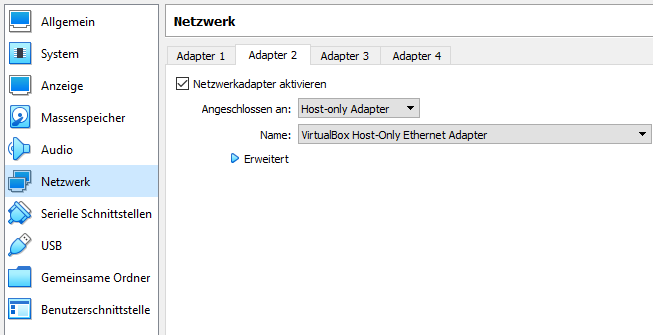
\includegraphics[scale=0.75]{images/vm-nw.png}
  \caption{Host-only Adapter}
\end{figure} \noindent
Es wird davon abgeraten ein eigenes NAT-Network zu konfigurieren, da in VirtualBox somit zwar eine Kommunikation zwischen den VMs funktioniert, jedoch keine Kommunikation zum Internet. 

\subsection{Server}
\subsection{Client}
\section{Technische Funktionalität} % Foto einfügen von VPN Tunneling? (von ko skripten)

